\section{Introduction}

\subsection{Purpose}

The purpose of this report is to provide a brief introduction into the current competition for Accenture, analyze those competitors, and evaluate potential competitors. Finally, this report will provide some insight as to how this analysis relates to the overall strategic planning process.

All firms face what \textcite{porterDynamicTheoryStrategy1991} deemed a ``longitudinal problem'' which is the dynamic process that provides the conditions wherein a competitive position can be created. In edition to this dynamic issue, \textcite{Porter1979} also noted the importance of understanding the present competitive landscape as part of the famous ``Five Forces'' model. For the purposes of understanding current and potential competitors, this report will not address the dyanmic create of competitive positions, but merely the existing and potential competitors at place in the market presently.

\subsection{Current Competitors}

Presently, the largest global competitors to Accenture PLC are: Capgemini, Tata, Cognizant, KPMG, and IBM.

\subsubsection{Capgemini}

Capgemini is a publically traded company with 270,000 employees operating in more than 50 countries. They are highly regarded in the European markets and should be seen primarily as a regional competitor to Accenture's European and Australian operations, though they are growing their global presence. Capgemini, like Accenture, provides a full suite of Technology consulting services, but is particularly known in the realms of Cybersecurtiy and IT Communications Service Providers. In this space, Capgemini is ranked in Gartner's 2020 ``Magic Quandrant'' for this market (Figure \ref{fig:itsc}).

\begin{figure}[h!]
  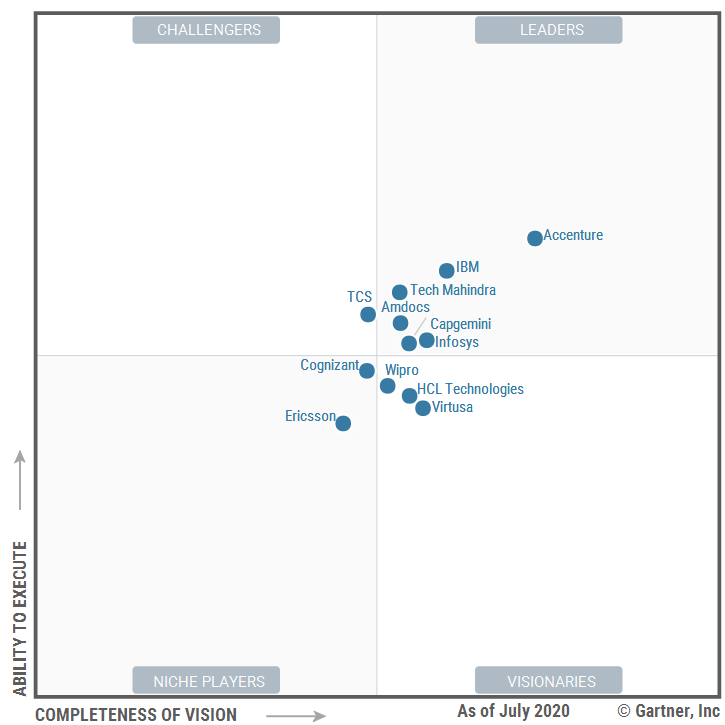
\includegraphics[width=\textwidth]{img/it_services_communications}
  \caption{Gartner's 2020 IT Services and Communications Magic Quandrant}
\label{fig:itsc}
\end{figure}

\subsubsection{Tata}

Tata Consultancy Services (TCS) is a private subsidiary of the private Indian based multinational conglomerate Tata Group. It is the largest consulting company in India. Tata operates in 46 countries. TCS has over 4 million employees, and is the largest private sector employer in India. Tata is a strong competitor for Accenture in the cloud infrastructure space, where Accenture is seeking new gowth (Figure \ref{fig:itci}). TCS' primarily competes with Accenture in the labor arbitrage space, offering to staff IT services in other nations from India. TCS excells at this.


\begin{figure}[h!]
  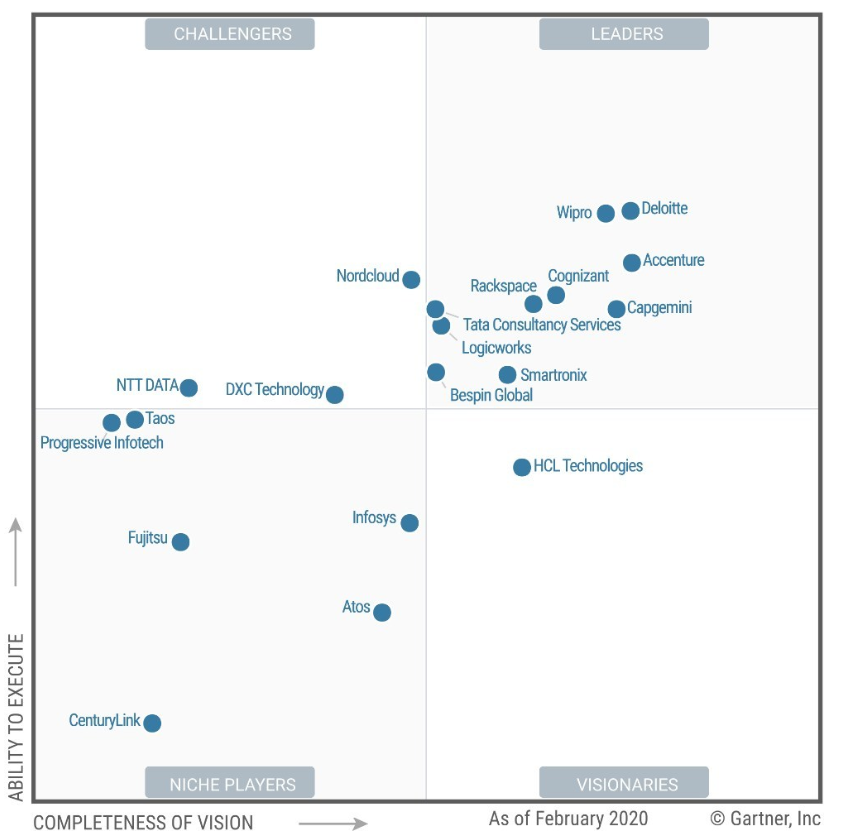
\includegraphics[width=\textwidth]{img/it_public_cloud}
  \caption{Gartner's 2020 IT Public Cloud Infrastructure Magic Quandrant}
  \label{fig:itpc}
\end{figure}


\subsubsection{Cognizant}

Cognizant is a public, American based consultancy firm. Cognizant competes with Accenture across the entire technology spectrum with their 281,000 employees. Cognizant competes in roughly 50 countries. Importantly for Accenture, Cognizant is also highly regarded in the Cloud Infrastructure space (Figure \ref{fig:itpc}), and like TCS presents a significant threat in this area. Cognizant, as a company, however, is burdened with a significant number of corporate scandals, including some fairly serious corruption issues. This limits their ability to compete against Accenture for business with companies in highly regulated industries.


\subsubsection{KPMG}

KPMG is a multinational professional services company that includes techology capabilities within their offerings. KPMG is primarily an advisory and financial auditing firm. They are based out of the Netherlands and are considered one of the ``Big Four'' accounting firms. KPMG employees 220,000 people across 147 countries. KPMG is one of the strongest competitor that Accenture faces in the data and analytics space (Figure \ref{fig:itda}). This area is considered critical to Accenture leadership for future growth. In addition to being a competitor, KPMG is also seen as a strategic partner. KPMG provides accounting and financial services to Accenture, and is Accenture will on occassion recommend KPMG services to clients in csses where KPMG is better suited to the client's needs. This consideration is returned by KPMG.

\begin{figure}[h!]
  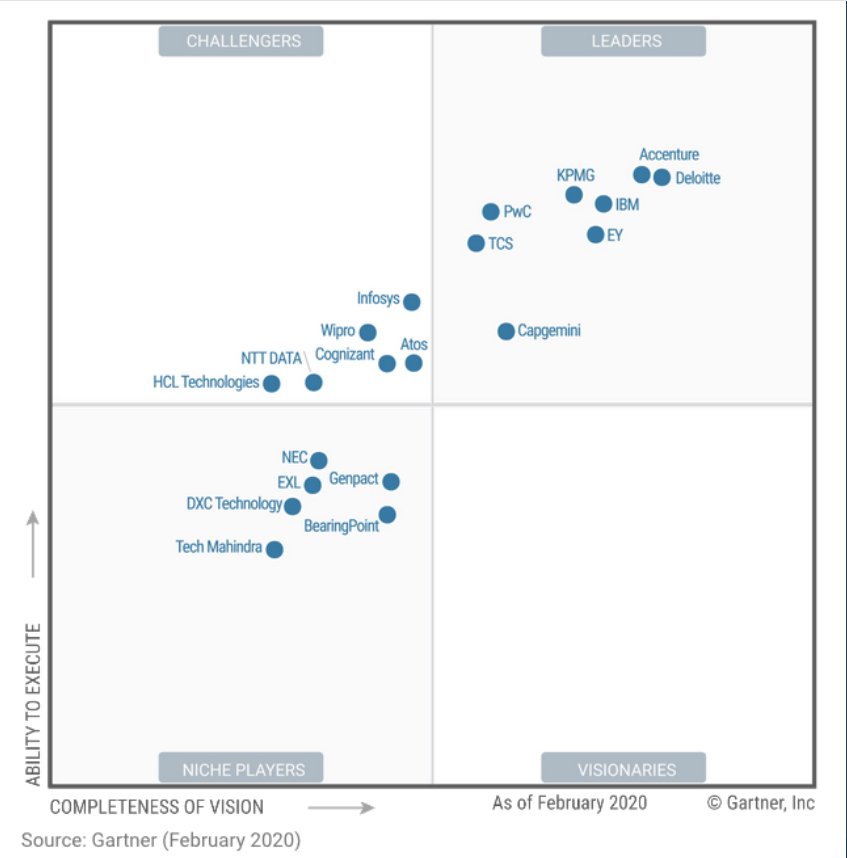
\includegraphics[width=\textwidth]{img/data_analytics}
  \caption{Gartner's 2020 Data Analytics Magic Quandrant}
  \label{fig:itda}
\end{figure}


\subsubsection{IBM}
IBM is a US based manufacturing, consulting, and research firm headquartered in the USA. They are a publically traded company with a presence in 177 countries, employing 352,000 people. IBM is a leader in many areas where Accenture is seeking to be the first choice for services (see figures \ref{fig:itsc, fig:itda}). IBM is also considered a strategic partner with Accenture. Accenture has numerous data analytics engagements that specifically include IBM Watson technology and/or IBM cloud technology implementations. In these cases, IBM becomes a supplier to Accenture's clients for the engagement.


\subsection{Analsys}

For the sake of this report, analaysis will focus on three specific competitors, Cognizant, KPMG, and IBM. For TCS, there is limited available public information, and what information that is available is of questionable quality. Further, TCS' primary area of competition with Accenture is in off-shoring IT Operations labor costs. This is a decreasing area of concentration for Accenture, and due to the scale differences between Accenture and TCS, Accenture is defitively not strong competition for Tata in this area. Rather, offshoring IT Operations is a service that Accenture provides to clients with whom Accenture has already provided other services. For Accenture this is a ``delighter'' function under the Kano model \parencite{xuCustomerRequirementAnalysis2007}. That is to say, Accenture offering this service will not likely win a customer from a competitor, but will provide a great deal of customer satisfaction after the sale when the customer finds that they appreciate the availability of the service. While TCS can not be said to not be a threat to Accenture, the vastly different approaches that they take towards provdiing Technology and Engineering services makes comparison difficult.


\begin{tiny}
% \usepackage{tablefootnote}
% \usepackage{array}
% \usepackage{pdflscape}
% \usepackage{longtable}


\begin{landscape}
\begin{longtable}{|>{\hspace{0pt}}p{0.208\linewidth}|>{\hspace{0pt}}p{0.235\linewidth}>{\hspace{0pt}}p{0.246\linewidth}>{\hspace{0pt}}p{0.25\linewidth}|}
\hline
\multicolumn{1}{|>{\hspace{0pt}}p{0.208\linewidth}}{} & \textbf{Cognizant}                                                                                                                                                                                                                                              & \textbf{KPMG}                                                                                                                                                                                                                                                           & \textbf{IBM}                                                                                                                                                                                                                                                                                                                    \endfirsthead
\cline{2-4}
\textbf{Products / Services}                          & \begin{tabular}{@{\labelitemi\hspace{\dimexpr\labelsep+0.5\tabcolsep}}l}Technology Implementation\\App Development\\\textbf{Cloud Infrastructure}\\Artificial Intelligence\\IT Consulting\\IT Services\\Management Consulting\\Systems Integration\end{tabular} & \begin{tabular}{@{\labelitemi\hspace{\dimexpr\labelsep+0.5\tabcolsep}}l}Business Products and Services\\Financial Services\\Audit\\\textbf{Data Analytics}\\Technology Implementation\\IT Consulting\\IT Services\\Management Consulting\\Outsourcing\end{tabular}      & \begin{tabular}{@{\labelitemi\hspace{\dimexpr\labelsep+0.5\tabcolsep}}l}Business Products and Services\\Technology Implementation\\Technology Research\\\textbf{Artificial Intelligence}\\\textbf{Data Analytics}\\\textbf{Cloud Infrastructure}\\\textbf{Cloud Services}\\IT Consulting\\IT Services\\IT Leasing\end{tabular}  \\
\cline{2-4}
\textbf{Market Ownership}                             & \begin{tabular}{@{\labelitemi\hspace{\dimexpr\labelsep+0.5\tabcolsep}}l}\$16.8B\end{tabular}                                                                                                                                                                    & \begin{tabular}{@{\labelitemi\hspace{\dimexpr\labelsep+0.5\tabcolsep}}l}\$29.8B\end{tabular}                                                                                                                                                                            & \begin{tabular}{@{\labelitemi\hspace{\dimexpr\labelsep+0.5\tabcolsep}}l}\$45.7B\tablefootnote{}\end{tabular}                                                                                                                                                                                                                    \\
\cline{2-4}
\textbf{What Provides Leverage?}                      & \begin{tabular}{@{\labelitemi\hspace{\dimexpr\labelsep+0.5\tabcolsep}}l}Cloud Capacity\\"Low Cost" vendor\\Aggressive MA \\System Integration Capabilities\end{tabular}                                                                                         & \begin{tabular}{@{\labelitemi\hspace{\dimexpr\labelsep+0.5\tabcolsep}}l}"Big 4" Firm / Reputation\\Financial Capabilities\\Data Analytics Expertise\end{tabular}                                                                                                        & \begin{tabular}{@{\labelitemi\hspace{\dimexpr\labelsep+0.5\tabcolsep}}l}Global Reputation\\AI RD Depth\\Ownership of Watson\\Big Data Capability\\Cloud Capability\end{tabular}                                                                                                                                                 \\
\cline{2-4}
\textbf{What Price Advantage Do They Have?}           & \begin{tabular}{@{\labelitemi\hspace{\dimexpr\labelsep+0.5\tabcolsep}}l}Extensively uses Offshore based labor\\Temporary worker visas~ \\Lower investment in Training\\Lower investment in RD\\Lower investment in Client Development\end{tabular}              & \begin{tabular}{@{\labelitemi\hspace{\dimexpr\labelsep+0.5\tabcolsep}}l}Price Competitive with Accenture\end{tabular}                                                                                                                                                   & \begin{tabular}{@{\labelitemi\hspace{\dimexpr\labelsep+0.5\tabcolsep}}l}Tends to be more costly than Accenture. \\\begin{tabular}[c]{@{}l@{}}Utilizes Electrical Engineers for functions \\that Accenture utilizes technology analysts\\ to do. \end{tabular}\end{tabular}                                                      \\
\cline{2-4}
\textbf{~Current Financial Position?}                 & \begin{tabular}{@{\labelitemi\hspace{\dimexpr\labelsep+0.5\tabcolsep}}l}Moderate Debt to Equity Ratio\\\$1.8B Net Income (2019)\end{tabular}                                                                                                                    & \begin{tabular}{@{\labelitemi\hspace{\dimexpr\labelsep+0.5\tabcolsep}}l}Very Low Debt to Equity Ratio\\Net Income due to IT Consulting is unknown\end{tabular}                                                                                                          & \begin{tabular}{@{\labelitemi\hspace{\dimexpr\labelsep+0.5\tabcolsep}}l}Moderate Debt to Equity Ratio\\\$9.4B Net Income (2019)\end{tabular}                                                                                                                                                                                    \\
\cline{2-4}
\textbf{What Next?}                                   & \begin{tabular}{@{\labelitemi\hspace{\dimexpr\labelsep+0.5\tabcolsep}}l}Invest heavily into cloud capability\\Market to cloud capability\\Continue to push low-cost selling points\\Continue acquisition strategy\end{tabular}                                  & \begin{tabular}{@{\labelitemi\hspace{\dimexpr\labelsep+0.5\tabcolsep}}l}Grow Big Data capability\\Grow Data Analytics capability\\\begin{tabular}[c]{@{}l@{}}Continue to leverage Financial Services \\capacity to drive data analytics sales\end{tabular}\end{tabular} & \begin{tabular}{@{\labelitemi\hspace{\dimexpr\labelsep+0.5\tabcolsep}}l}\begin{tabular}[c]{@{}l@{}}Heavily market strong AI and Data analytics\\ capability\end{tabular}\\Rely upon market reputation\\Leverage patent portfolio\\Grow Cloud Infrastructure\\Grow Leasing Capacity\end{tabular}                                 \\
\hline
\end{longtable}
\end{landscape}
\end{tiny}

For Capgemini, they are primarily a regional competitor to Accenture. While they are making headway into the USA, they really are not yet a globally competitive player. This does not mean that Accenture can ignore them. They do, after all, present a legitimate threat to Accenture's European expansion goals. However, due to the fact that they are more regional, and this analysis is focused on global comeptitors, they will be excluded from further analysis.

Accenture has identified several areas of future focused growth. Specifically called out in the 2019 Annual Report are Data analytics capabilities, Aritifical Intelligence and Automation, and Big Data initiatives. Additionally, in September of 2020, the CEO announced a \$3B investment into Accenture's ``Cloud First'' initiative \parencite{AccenturePLC2019,AccentureCloudFirst2020}. It is obvious from the Gartner analysis \parencite[][see Figures 1-3]{gartnerinc.StrategicPlanning2020a} of these competitors that they each represent strong competitors in areas that Accenture has specifically targeted as strategic opportunities.
